\section{}
For a thin cantilever, the stress function is given by
\begin{align*}
    \Phi = -c_1xy + \frac{c_2x^3}{6} - \frac{c_3x^3y}{6} - \frac{c_4xy^3}{6} - \frac{c_5x^3y^3}{9} - \frac{c_6xy^5}{20}
\end{align*}
\begin{figure}[h]
    \centering
    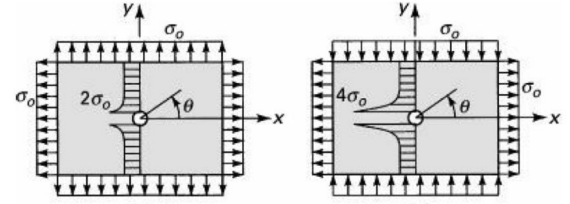
\includegraphics[width=0.35\linewidth]{Questions/Figures/Q4ProblemDiagram.png}
    \caption{Problem diagram for Question 4.}
    \label{fig:Q4ProblemDiagram}
\end{figure}
Determine the stresses $\sigma_x$, $\sigma_y$, and $\tau_{xy}$ by using the elasticity method.

I am not doing this by hand. 

With Matlab
\lstinputlisting[language=Matlab]{Questions/q4.m}

This solves for the constants as 
\begin{verbatim}
>> sol

sol = 

  struct with fields:

    c1: -(p0*x^2)/(4*L*h*t)
    c2: -p0/(2*L*t)
    c3: -p0/(L*h*t)
    c4: (6*p0*x^2)/(L*h^3*t)
    c5: 0
    c6: 0

>> 
\end{verbatim}

and the stresses as
\begin{verbatim}
sigma_x =
 
- (2*c5*x^3*y)/3 - c6*x*y^3 - c4*x*y
 
 
sigma_y =
 
c2*x - (2*c5*x*y^3)/3 - c3*x*y
 
 
tau_xy =
 
c5*x^2*y^2 + (c3*x^2)/2 + (c6*y^4)/4 + (c4*y^2)/2 + c1
\end{verbatim}